% Giacomo Petrillo
% lezione di Morello

\section{Assiomi e proprietà elementari}
\label{sec:assiomi}

\begin{definition}[Probabilità]
	Definiamo in astratto la probabilità $\fundef[P]{\pset(S)}\R$ come funzione dai sottoinsiemi\footnote{%
	In verità la probabilità è definita su una $\sigma$-algebra, non sull'insieme delle parti.
	In generale non si può ricondurre una $\sigma$-algebra a un insieme delle parti;
	ad esempio la $\sigma$-algebra generata dagli aperti di $\R$
	contiene tutti i punti di $\R$ ma non è l'insieme delle parti.
	Comunque per il livello di approfondimento che raggiungeremo
	andrà sempre bene pensare alla probabilità come definita su un insieme delle parti.}
	di un \emph{insieme universo} $S$ a valori reali, che soddisfa i seguenti \emph{assiomi di Kolmogorov}:
	\begin{enumerate}
		\item La probabilità è non negativa:
		\[\forall A\subseteq S:P(A) \ge 0;\]
		\item La probabilità dell'unione di una famiglia numerabile di sottoinsiemi disgiunti due a due
		è la somma delle probabilità:
		\begin{align*}
			\forall \mathcal F\subseteq \pset(S):
			\#\mathcal F\le \#\N,\ 
			\forall A,B\in\mathcal F: A\cap B=\emptyset \rightarrow \\
			\rightarrow P\left(\bigcup\mathcal F\right)=\sum_{A\in\mathcal F}P(A);
		\end{align*}\label{kolm2}
		\item La probabilità di tutto è unitaria:
		\[P(S)=1.\]
	\end{enumerate}
\end{definition}

\begin{theorem}[Probabilità dell'unione]
	$P(A\cup B) = P(A) + P(B) - P(A\cap B)$.
\end{theorem}

\begin{proof}
	Scrivo $B$ come l'unione di due insiemi disgiunti:
	\[B = (A\cap B) \cup (\comp A \cap B)\]
	dove $\comp A\is S\setminus A$; per l'assioma \ref{kolm2} segue
	\begin{equation}
		\label{eq:pdib}
		P(B) = P(A\cap B) + P(\comp A \cap B).
	\end{equation}
	Scrivo $A\cup B$ come l'intersezione di se stesso con $S=A\cup\comp A$
	\[A\cup B = (A\cup\comp A) \cap (A\cup B)\]
	e applico la proprietà distributiva
	\begin{align*}
		A\cup B
		&= (A\cap A) \cup (A\cap B) \cup (\comp A\cap A) \cup (\comp A \cap B) = \\
		&= A \cup (\comp A\cap B)
	\end{align*}
	che sono disgiunti, da cui segue
	\begin{align}
		P(A\cup B)
		&= P(A) + P(\comp A\cap B) \implies \notag \\
		\implies P(\comp A\cap B)
		&= -P(A) + P(A\cup B). \label{eq:pdicacb}
	\end{align}
	Sostituendo la \eqref{eq:pdicacb} nella \eqref{eq:pdib} ottengo la tesi.
    La \autoref{fig:sets} illustra graficamente la dimostrazione.
    %
    \begin{figure}
        %
        \centering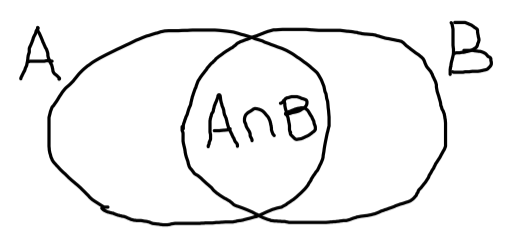
\includegraphics[width=10em]{sets}%
        %
        \caption{Sommando la probabilità di $A$ e $B$, la probabilità di
        $A \cap B$ viene contata due volte, quindi va sottratta per ottenere
        la probabilità di $A \cup B$.} \label{fig:sets}
        %
    \end{figure}
    %
\end{proof}

\begin{definition}[Probabilità condizionata]
	Sia $P(C)\neq 0$. Definiamo la \emph{probabilità di $A$ dato $C$} come
	\[P(A|C) \is \frac{P(A\cap C)}{P(C)}.\]
\end{definition}

\noindent Il senso della probabilità condizionata è che se $C$ diventa certo
devo modificare le probabilità degli altri insiemi in modo che il nuovo insieme universo sia $C$.

\begin{exercise}
	Verificare che gli assiomi di Kolmogorov continuano a valere se, per fissato $C$, sostituisco in generale $P(X)$ con $P(X|C)$.
\end{exercise}

\begin{definition}[Indipendenza]
	$A$ e $B$ sono \emph{indipendenti} se $P(A|B) = P(A)$,
	oppure se almeno uno dei due è l'insieme vuoto.
\end{definition}

\begin{exercise}
	$A$ e $B$ sono indipendenti se e solo se $P(A\cap B) = P(A)P(B)$.
\end{exercise}

\begin{exercise}
	Siano $P(A)=\frac1{10}$ e $P(B)=1$, $A$ e $B$ sono indipendenti?
\end{exercise}

\begin{solution}
	Sono indipendenti, perché:
	\begin{align*}
		&1 \ge P(A\cup B) \ge P(B) = 1 \\
		\implies &1 = P(A\cup B) = P(A) + P(B) - P(A\cap B) = \frac{11}{10} - P(A\cap B) \\
		\implies &P(A\cap B) = \frac{1}{10} \\
		&P(A|B) = \frac{P(A\cap B)}{P(B)} = \frac{\frac{1}{10}}{1} = P(A).
	\end{align*}
\end{solution}

\begin{exercise}
	Siano $A$ e $B$ mutualmente esclusivi. Dire cosa significa e se allora sono indipendenti.
\end{exercise}

\begin{solution}
	Significa che $A\cap B=\emptyset$ e in generale non implica l'indipendenza, perché si ha sempre $P(A|B)\propto P(A\cap B)=0$.
\end{solution}
